\section{Single fluid description of dusty gas}\label{setup} 
We model an accretion disk as a mixture of gas with dust treated as a 
pressureless fluid. We denote their density and
velocity field as $(\rhog,\bm{v}_\mathrm{g})$ and
$(\rhod,\bm{v}_\mathrm{d})$, respectively. The mixture has a single 
temperature $T$, and the mixture pressure $P$ arise solely from the 
gas component.  

The two fluids interact via a drag force parameterized by a stopping
time $\tstop$ 
such that 
\begin{align}  
  \rhod\left.\frac{\p \bm{v}_\mathrm{d}}{\p t}\right|_\mathrm{drag}= -
  \rhog\left.\frac{\p \bm{v}_\mathrm{g}}{\p t}\right|_\mathrm{drag}=
  - \frac{\rhog\rhod}{\left(\rhod+\rhog\right)}\frac{\left(\bm{v}_\mathrm{d} -
    \bm{v}_\mathrm{g}\right)}{\tstop}. 
\end{align}
is the dust-gas friction force per unit volume. Note that $\tstop$ 
differs slightly from the stopping time $\tau_\mathrm{s} =
\tstop\rhog/\left(\rhog+\rhod\right)$ defined in previous studies
\citep[e.g.][]{youdin05a,jacquet11}.   

We consider the limit of tightly-coupled dust particles with 
$\tstop\OmK\ll 1 $, where $\OmK$ is the Keplerian orbital
frequency. This allows us to simplify the problem by using the
`terminal velocity approximation' so that the dust-gas velocity
difference is 
\begin{align}
  \bm{v}_\mathrm{d} - \bm{v}_\mathrm{g} = \frac{\nabla
    P}{\rhog}\tstop, 
\end{align}
\citep{youdin05a,jacquet11}. 

%In the limit of strong dust-gas drag (stopping time $\tstop\to 0$) 
In this limit of strong dust-gas drag, \cite{laibe14} give a single
fluid description of the mixture: 
\begin{align}
  &\frac{D\rho}{Dt} = -\rho\nabla\cdot\bm{v}, \label{masseq}\\ 
  &\frac{D\bm{v}}{Dt} = - \nabla\Phi - \frac{1}{\rho}\nabla  P, \label{momeq}\\ 
  &\frac{D\tepsilon}{Dt} = -\frac{1}{\rho} \nabla \cdot \left(\tepsilon 
  \tstop \nabla P \right),\label{dusteq}\\
  &\frac{D T}{D t} = - \left(\gamma-1\right)T\nabla\cdot\bm{v} +
  \mathcal{H}_\mathrm{drag} + \mathcal{H}_\mathrm{eff}  - \Lambda, \label{tempeq} 
\end{align}
where $D/Dt \equiv \p_t + \bm{v}\cdot\nabla$ is the Lagragian
derivative \emph{following the mixture} with center-of-mass velocity  
\begin{align}
  \bm{v} \equiv \frac{\rhog\bm{v}_\mathrm{g} + 
    \rhod\bm{v}_\mathrm{d}}{\rho}, 
\end{align}
and 
\begin{align}
  \rho \equiv \rhog + \rhod
\end{align}
is the total mixture density. For an ideal gas the pressure is given
by $P = \mathcal{R}\rhog T/\mu $, where $\mathcal{R}$ is
the gas constant and $\mu$ is the mean molecular weight. 

In Eq. \ref{dusteq}, 
\begin{align}
  \tepsilon \equiv \frac{\rhod}{\rho}  = \frac{\epsilon}{1+\epsilon} 
\end{align}
is the dust-fraction and $\epsilon=\rhod/\rhog$ is the usual
dust-to-gas ratio. Note that Eq. \ref{dusteq} is 
equivalent to Eq. 46 of \cite{jacquet11}. 

For the mixture's temperature evolution, Eq. \ref{tempeq}, $\gamma$ is
the adiabatic index; $\mathcal{H}_\mathrm{drag}$ represents heating
due to dust-gas drag and $\mathcal{H}_\mathrm{eff}$ is an effective
energy source arising from transforming from the two-fluid to
one-fluid description \citep[see][ for details]{laibe14}. We also
include a simple model of radiative cooling,
\begin{align}
  \Lambda = \frac{T -
    T_\mathrm{ref}}{t_\mathrm{cool}}, \label{realenergy} 
\end{align}
which relaxes the mixture back to a prescribed temperature profile   
$T_\mathrm{ref}$ on a timescale of $\tcool$. We will shortly simplify
the problem by considering rapid cooling, $\tcool\to0$. 


For the disk problem the external potential $\Phi$ is  
that for a star of mass $M_*$, 
\begin{align}\label{thin_disk_potential}
  \Phi(r,z) =-\frac{GM_*}{\sqrt{r^2 + z^2}}\simeq
  -\frac{GM_*}{r}\left(1 - \frac{z^2}{2r^2}\right), 
\end{align}
where $G$ is the gravitational constant, and $(r,\phi, z)$ are
cylindrical co-ordinates centered on the star. 
The second equality is the 
thin-disk approximation for the disk potential, appropriate for
$|z|\ll r$. We shall adopt this approximate potential in order to
obtain analytic expressions for the disk equilibria.  

\subsection{Locally isothermal equation of state}\label{loc_iso_eos}
For later comparison it is convenient to re-write the temperature
evolution, Eq. \ref{tempeq}, to that for the pressure: 
\begin{align}
  \frac{\p P}{\p t} + \bm{v}_\mathrm{g}\cdot\nabla P = - \gamma P
  \nabla\cdot \bm{v}_\mathrm{g}  + \mathcal{H} 
%\frac{\rho \mathcal{R}}{\mu}\frac{T
%  - T_\mathrm{ref}}{t_\mathrm{cool}}, \label{realenergy}
\end{align}
where $\mathcal{H}$ collects together dust-drag heating and radiative
cooling. 

We now simplify the gas energy equation by considering short cooling 
times $\tcool\to 0$, appropriate for the outer parts of an irradiated
protoplanetary disk \citep{chiang97,lin15}. Then the disk temperature
$T = T_\mathrm{ref}$ at all times, and so we may
adopt a locally isothermal equation of state 
\begin{align}\label{eos}
  P = c_s^2(r,z)\rhog = c_s^{2}(1 - \tepsilon)\rho,   
\end{align}
where $c_s(r,z)= \sqrt{\mathcal{R}T_\mathrm{ref}/\mu}$ is a prescribed
sound-speed profile fixed in time.  

In practice we consider vertically 
isothermal disks with \begin{align}\label{power_temp}
  c_s^2(r) \propto r^{q},
\end{align}
where $q$ is the power-law index for the disk temperature. For $q=0$
the disk is strictly isothermal. 

If we define the effective sound-speed $c_{s,\mathrm{eff}} = c_s\sqrt{\left(1 -
    \tepsilon\right)}$, then the equation of state has the standard
form $P=c_{s,\mathrm{eff}}^2\rho$. Since the dust-fraction $\tepsilon$
typically decrease away from the midplane, we expect vertically
isothermal dusty disks to in fact behave as if it
had a temperture \emph{increasing} away from $z=0$.   

\subsection{Effective energy equation}
Although we have eliminated the need of an evolutionary energy
equation (Eq. \ref{realenergy}) by choosing a locally isothermal
equation of state (Eq. \ref{eos}), we show that the mixture 
nevertheless obeys an effective evolutionary energy equation. This is
because advection of the dust-fraction, described by
Eq. \ref{dusteq}, can be transformed into an energy-like 
equation. We 
%We show that for a prescribed temperature distribution, the mixture
%obeys an evolutionary energy equation, due to the advection of the
%dust-fraction. 
eliminate $\tepsilon$ in favor of $P$, 
\begin{align*}
  \tepsilon = 1 - \frac{P}{c_s^2(r,z)\rho}, 
\end{align*}
then Eq. \ref{dusteq} becomes
\begin{align}
%\frac{DP}{Dt} 
\frac{\p P}{\p t} + \bm{v}\cdot\nabla P  
&= - P \nabla\cdot\bm{v} + P\bm{v}\cdot\nabla\ln{c_s^2}
                + \mathcal{C},  \label{eff_energy} \\
\mathcal{C}&\equiv c_s^2 \nabla\cdot\left[\tstop\left(1 -
  \frac{P}{c_s^2\rho}\right)\nabla 
  P\right].
\end{align}
Comparing with Eq. \ref{realenergy}, we see that 
Eq. \ref{eff_energy} is the energy equation for an ideal gas of
adiabatic index $\gamma=1$, but now with the imposed temperature
gradient $\nabla c_s^2$ and dust-gas drag $\mathcal{C}$ playing the
role of radiative cooling ($\Lambda$ in 
Eq. \ref{realenergy}). 

%In this form, the function $\mathcal{C}$ can be interpreted
%as a cooling term.    
If we denote 
\begin{align}
  \bm{F} \equiv  - \frac{\nabla P}{\rho}
\end{align}
for the pressure forces, then
\begin{align*}
  \mathcal{C} = - c_s^2\nabla \left( \tepsilon \tstop \rho \bm{F}
  \right), 
\end{align*}
which is in the same form as cooling by radiative diffusion. In protoplanetary
disks the heat flux, proportional to $\bm{F}$, is directly radially
outwards and vertically upwards. This is simply a reflection of
particle drift (inwards and downwards). Particle flux into a region contributes
to `cooling' of that region because the effective temperature is
lowered. 

Eq. \ref{eff_energy} can be written in conservative form,
\begin{align*}
  \frac{\p P}{ \p t} + \nabla\cdot\left\{P\left[\bm{v} -
      \tstop\left(c_s^2 - \frac{P}{\rho}\right)\nabla\ln{P}\right]
    \right\}\\
  = \left[P\bm{v} - \tstop\left(c_s^2 - \frac{P}{\rho}\right)\nabla
    P\right]\cdot\nabla\ln{c_s^2}. 
\end{align*} 
We may thus re-interpret $P$ as the mixture's energy density, but the
energy flux has an additional contribution from the pressure
gradient and dust-gas friction. The term on the right-hand-side, owing
to the imposed temperature profile, can be interpreted as an external
heat source.  

%We comment that 

\subsection{Entropy of an isothermal dusty gas }

The gas component of the mixture has a specific entropy
$S = C_p\ln{\left(P^{1/\gamma}/\rhog\right)}$, where $C_p$ is the heat capacity at constant
pressure. However, this is not a useful quantity for (locally)
isothermal gas. 

Nevertheless, since we have shown that an isothermal dusty gas
effectively has $\gamma=1$ we can define an effective (dimensionless)  
entropy for the \emph{entire mixture} as 
\begin{align}
   \seff \equiv \ln \frac{P}{\rho} = \ln{\left[c_s^2(1-\tepsilon)\right]}.  
\end{align} 
We shall see that by defining an effective entropy this way, many of the 
results concerning the stability of dusty gas will have identical form
and interpretations to that in standard adiabatic hydrodynamics of 
pure gas. For example, if $c_s^2$ is constant and $\tstop=0$, then
$D\seff/ D t = 0$ since $D\tepsilon/D t=0$ in that case.  

The physical reason for this analogy is that with strong drag, the dust is almost
perfectly entrained in the gas flow, but there is some gain/loss of 
dust particles between different gas parcels if dust-gas
friction if finite. This property is analogous to the entropy of an adiabatic
pure gas subject to heating/cooling: entropy is conserved following
a gas parcel, except if there is heat exchange between a fluid parcel
and the surrounding.  

\section{Dynamical equilibria}\label{eqm}
 
For a given distribution of the dust-fraction $\tepsilon$ (or
dust-to-gas ratio $\epsilon$), the 
mass and momentum Eqs. \ref{masseq}---\ref{momeq} admit     
axisymmetric steady states with $\rho(r,z)$ and 
$\bm{v}=r\Omega(r,z)\hat{\bm{\phi}}$ where $\Omega = v_\phi/r$, which satisfy 
\begin{align}
  r\Omega^2 &= \frac{\p \Phi}{\p r} + \frac{1}{\rho}\frac{\p P}{\p
    r},\label{steady_momr}\\
  0 & = \frac{\p\Phi}{\p z} + \frac{1}{\rho}\frac{\p P}{\p z},\label{steady_momz}
%  0 & = \nabla\cdot\left(\tepsilon\tstop\nabla P\right) \label{steady_dust}
\end{align}
with $P=P(\tepsilon,\rho)$ given by the equation of state
(Eq. \ref{eos}). An explicit solution is presented in
\S\ref{steady_state}.  
However, disk structures obtained this way generally do not satisfy 
the steady state effective energy Eq. \ref{eff_energy} because
$\mathcal{C}\neq0$ for general solutions to
Eq. \ref{steady_momr}---\ref{steady_momz}. 

In practice the dust particles settle vertically on a timescale 
$t_\mathrm{settle}\sim 1/\OmK^2\tstop$, although for tightly-coupled dust
particles this is much longer than that to establish vertical
hydrostatic equilibrium in the gas component ($\sim 1/\OmK$).  
True steady states may be calculated by invoking an underlying gas
turbulence, which leads to dust diffusion \citep{takeuchi02, youdin07, 
 lyra13}. This complication is beyond the scope of this paper. 

In this work, we will assume that $\tstop$  is sufficiently small so
that settling occurs on much longer timescales  than that of interest; or
consider equilibria with $\mathcal{C}\equiv 0$, namely   
\begin{inparaenum}[1)] 
\item 
  unstratified disks with finite dust-gas drag (\S\ref{si});  
\item 
  perfectly-coupled dust with $\tstop=0$ (\S\ref{results}). 
\end{inparaenum} 
Vertical settling is absent in both cases. 


%Eq. \ref{steady_dust} makes it difficult to obtain equilibrium
%solutions explicitly. However, if the diffusive process is slow and
%can be neglected, then one may just solve
%Eq. \ref{steady_momr}---\ref{steady_momz} with a prescribed (initial)
%distribution of the dust fraction $\tepsilon(r,z)$. 

\subsection{Disk structure with a prescribed dust distribution}\label{steady_state}  
To obtain an actual disk structure for numerical computations, we
assume a Gaussian profile in the dust-to-gas ratio,   
\begin{align}\label{dust_gauss}
  \epsilon(r,z) = \epsilon_0(r)
  \exp{\left[-\frac{z^2}{2\Htilde^2(r)}\right]}. 
\end{align}
%For simplicity we assume the dust-to-gas ratio at the mid-plane
%$\epsilon_0$, as well as its characteristic scale-height
%$\widetilde{H}$, are both constant.
% We take the mid-plane dust-to-gas ratio
%to be a power-law in radius,  
%\begin{align}
%  \epsilon_0(r) = \epsilon_{00}\left(\frac{r}{r_0}\right)^{-d},  
%\end{align}
%where $\epsilon_{00}$ is the dust-to-gas ratio at the fiducial radius
%$r_0$.  
Inserting Eq. \ref{dust_gauss} into vertical hydrostatic equilibrium,
Eq. \ref{steady_momz} and integrating with the approximate
gravitational potential (Eq. \ref{thin_disk_potential}) we obtain the
gas density as
\begin{align}
  &\rhog(r,z)= \notag\\
&\rho_\mathrm{g0}(r)\exp{\left\{ - \frac{z^2}{2\Hgas^2}
    -\epsilon_0\frac{\Htilde^2}{\Hgas^2}\left[1 -
      \exp{\left(-\frac{z^2}{2\Htilde^2}\right)}\right] \right\}}, 
\end{align}
where
\begin{align}
  \Hgas = \frac{c_s}{\OmK}, \quad \OmK \equiv \sqrt{\frac{GM_*}{r^3}},   
\end{align}
is the gas scale-height in the dust-free limit and $\OmK$ is the
Keplerian frequency, respectively. 

We usually consider gas-dominated disks with $\epsilon_0 \ll 1$.  
Then $\rhog(r,z)$ is effectively Gaussian, as in the 
dust-free case. The dust density is approximately 
\begin{align}
  \rhod \simeq \epsilon_0\rho_\mathrm{g0}(r) \exp
        {\left(-\frac{z^2}{2H_\mathrm{d}^2}\right)}, 
\end{align}
with 
\begin{align}
  \frac{1}{H_\mathrm{d}^2} = \frac{1}{\Htilde^2} + \frac{1}{\Hgas^2}, 
\end{align}
and $H_\mathrm{d}$ is the dust-scale height. In numerical
calculations, we  we specify $H_\mathrm{d}< \Hgas$ to obtain 
$\Htilde$ for input. 

Finally, we define 
\begin{align}
  Z \equiv \epsilon_0\frac{\Hd}{\Hg} \simeq
  \frac{\Sigma_\mathrm{d}}{\Sigma_\mathrm{g}} 
\end{align}
as a measure of the local metalicity, where $\Sigma_\mathrm{d}$ and
$\Sigma_\mathrm{g}$ are the dust and gas surface densities,
respectively. The second equality holds for $\epsilon_0\ll1$.  

%\Sigma_\mathrm{d}$ and the gas
%surface density $\Sigma_\mathrm{g}$.  

\subsection{Orbital frequency} 
In the thin-disk approximation, the disk orbital frequency is 
\begin{align}
  \Omega(r,z) = \OmK(r)\left[1 - \frac{3}{2}\frac{z^2}{r^2} +
    \frac{h_\mathrm{g}^2}{\left(1+\epsilon\right)}\frac{\p}{\p\ln{r}}\ln{\left(c_s^2\rhog\right)}
    \right]^{1/2}, 
\end{align}
where 
\begin{align}
  h_\mathrm{g} \equiv \frac{\Hgas}{r}
\end{align}
is the characteristic disk aspect-ratio. 

\subsection{Vertical shear}\label{vertshear}
The mixture possess vertical shear. To see this, we eliminate $\Phi$
between Eq. \ref{steady_momr}---\ref{steady_momz} to 
obtain 
\begin{align}\label{vshear}
  r\frac{\p \Omega^2}{\p z} 
%&= \frac{\p\ln{\rho}}{\p r}\frac{\p}{\p
%    z}\left[c_s^2(1-\tepsilon)\right] - \frac{\p\ln{\rho}}{\p z}
%  \frac{\p}{\p r} \left[c_s^2(1-\tepsilon)\right]\\  
   = \frac{1}{\rho}\left(\frac{\p P}{\p r}\frac{\p \seff}{\p z} -\frac{\p
    P}{\p z}\frac{\p \seff}{\p r} \right). 
\end{align}
Writing Eq. \ref{vshear} in terms of the gas density and dust-to-gas
ratio with a power-law temperature profile (Eq. \ref{power_temp}) gives 
\begin{align}\label{vshear2}
  &r\frac{\p \Omega^2}{\p z}  =
  \frac{c_s^2(r)}{\left(1+\epsilon\right)^2}\left\{
  \frac{\p\epsilon}{\p r}\frac{\p\ln{\rhog}}{\p z}
%  -\frac{\p\epsilon}{\p z}\left[\frac{\p\ln{\rhog}}{\p r} + \frac{q}{r}\right]\right.\notag\\
 -\frac{\p\epsilon}{\p z}\frac{\p\ln{P}}{\p r}\right.\notag\\
  &\phantom{ r\frac{\p \Omega^2}{\p z}  =
    \frac{c_s^2(r)}{\left(1+\epsilon\right)^2}\left\{\right\} }
  \left. -\frac{q}{r} \left(1+\epsilon\right)\frac{\p\ln{\rhog}}{\p z} \right\} 
\end{align}
The first two terms correspond to vertical shear caused by spatial
variations in the dust-to-gas ratio; while the third term
proportional to $q$ corresponds to vertical shear due to the 
radial temperature gradient. The last term survives in the dust-free
limit. 

We can compare these sources by 
evaluating them using the equilibrium
solutions in \S\ref{steady_state}. We assume the disk is radially
smooth so that $\p_r\sim 1/r$, and the dust-to-gas ratio
$\epsilon\ll1$. This gives 

\begin{align}\label{vshear_split}
  \frac{\left|r\p_z\Omega\right|_{\text{
        dust/gas gradient}}}{\left|r\p_z\Omega\right|_{\text{
        temp. gradient}}} \sim
 % \epsilon \frac{\mathrm{max}\left(\delta^2,
  %  1\right)}{\left|q\right|\left(\epsilon + \delta^2\right)},
 \epsilon \frac{\mathrm{max}\left(\delta^2,
    1\right)}{\left|q\right|\left(1+\epsilon\right)\delta^2},
\end{align}
where $\delta\equiv \Htilde/\Hgas$. 
Since $|q|=O(1)$ in PPDs, Eq. \ref{vshear_split} indicates that
vertical shear due to variations in the dust-to-gas ratio dominates 
over that due to the radial temperature gradient for thin dust layers
such that $\delta^2\ll \epsilon$. Otherwise, vertical shear is
associated with $\p_rc_s^2$.  

\subsection{Vertical buoyancy}\label{vbuoyancy}
Having identified the entropy of an isothermal dusty gas, we find the
vertical buoyancy frequency $N_z$ of the mixture is given by 
\begin{align}
  N_z^2 \equiv - \frac{1}{\rho}\frac{\p P}{\p z}\frac{\p \seff}{\p z} &=
  \frac{c_s^2(r)}{\left(1+\epsilon\right)^2}\frac{\p\ln\rhog}{\p 
  z}\frac{\p\epsilon}{\p z} \\ &
                                  =
  \frac{\epsilon}{\left(1+\epsilon\right)^2}\left(\frac{z}{\Htilde}\right)^2\OmK^2\notag,  
\end{align}
where the second equality assumes $c_s=c_s(r)$ and the final equality
applies to the equilibria in \S\ref{eqm}. Thus,  
\begin{align*}
N_z\lesssim
O\left(\sqrt{\epsilon_0}\OmK\right). 
\end{align*}
However, for thick dust layers such that $H_\epsilon \gg \Hg$, 
$\mathrm{max}\left(N_z\right)$ may occur outside a finite vertical domain.  


 % N_z^2 
%\end{align}

\section{Limiting behaviours}\label{limits}

In this section we review the basic properties of the 
single-fluid mixture using Eqs.\ref{masseq}--\ref{momeq} with 
Eq. \ref{eff_energy} in place of the dust continuity equation. Our
discussion is based on the corresponding axisymmetric linearized
equations. A variable $f$ is
subject to Eulerian perturbations of the form 
\begin{align}
 \real\left[ \delta f(r,z)\exp{\left(-\ii\sigma t\right)}\right], 
\end{align}
where $\sigma$ is the complex mode frequency. For later convenience we
write 
\begin{align}
  \sigma = \ii s - \omega,
\end{align}
where $s$ and $\omega$ are the growth rate and real frequencies,
respectively. Thus perturbations have time dependence $e^{st +
  \ii\omega t}$.  

In Appendix
\ref{var_prin} we derive the integral relation,  
\begin{align}
%&  \sigma^2\int\rho\left(|\dd v_r|^2 + |\dd v_z|^2\right)dV \notag\\
  \sigma^2\mathcal{I}^2
&= \int\left[ \rho
  |\dd v_r|^2A + \rho  \dd v_z \dd v_r^* B + \rho \dd v_z^*\dd v_r C +
  \rho |\dd v_z|^2 D\phantom{\frac{1}{1}}\right. \notag\\
&\phantom{===}  \left. + \frac{1}{P}\Bigl\lvert \nabla\cdot\left(P\dd
  \bm{v}\right)\Bigr\rvert^2\right]dV  -\int \left(\nabla\cdot\dd\bm{v}^*\right)\dd\mathcal{C}dV \notag\\
&\phantom{===}
- \int P
  \left(\nabla\cdot\dd\bm{v}^*\right)\left(\dd\bm{v}\cdot\nabla\ln{c_s^2}\right)dV.\label{int_rel}
\end{align} 
The real integral $\mathcal{I}^2>0$ and coefficients $A,B,C,D$ can be
read off Eq. \ref{integral_ex}. %Note that $B=C$ from dynamical equilibrium
%(Eq. \ref{vshear}). 
We now consider various limits of Eq. \ref{int_rel}.    


\subsection{Strictly isothermal gas perfectly coupled to dust}\label{iso_perfect}
When $c_s^2$ is a constant and $\tstop=0$, the dusty-gas equations are
exactly equivalent to that for adiabatic hydrodyamics with unit adiabatic
index. Although the gas is strictly isothermal, the mixture behaves 
adiabatically because the dust fraction $\tepsilon$ is advected with 
the gas. This is similar to entropy being conserved following an
adiabatic gas when there is no heating or cooling.  

In this case, the last two integrals in Eq. \ref{int_rel} vanish. Then 
requiring $\sigma^2>0$  gives the criteria 
for the axisymmtric \emph{stability} of an isothermal gas perfectly 
coupled to dust,  
\begin{align}
  \kappa^2 + c_s^2 \nabla\ln{\rhog}\cdot\nabla\tepsilon &> 0,\label{dusty_solberg1}  \\
  -c_s^2\frac{\p\ln{\rhog}}{\p z}\left(-\kappa^2\frac{\p\tepsilon}{\p
    z} + r\frac{\p\Omega^2}{\p z}\frac{\p \tepsilon}{\p r} \right) & > 0, \label{dusty_solberg2}
\end{align} 
%\begin{align}
%  \kappa^2 - \frac{1}{\rho}\nabla P \cdot \nabla s &> 0, \label{dusty_solberg1}    \\
%  -\frac{1}{\rho}\frac{\p P}{\p z} \left(\kappa^2 \frac{\p s}{\p z} -
%  r\frac{\p\Omega^2}{\p z}\frac{\p s}{\p r}\right) &>0, \label{dusty_solberg2}
%\end{align} 
where %$s = \ln{P/\rho}$, 
$\kappa^2 \equiv r^{-3}\p_r\left(r^4\Omega^2\right)>0$ is the 
square of the epicylic frequency. %We assume $\kappa^2>0$.  
Eq. \ref{dusty_solberg1}---\ref{dusty_solberg2} are in fact the 
the Solberg-Hoiland criteria for axisymmetric stability of adiabatic
gas if one inserts $C_p\ln{\left(1 -
    \tepsilon\right)}$ for the entropy in the standard
expression for said criteria \citep[e.g.]{tassoul78}.   


\subsubsection{Order-of-magnitude estimates} 
We evaluate the above stability criteria for the vertically-Gaussian
distributions for the gas density and the dust-to-gas ratio as 
described in \S\ref{eqm}. 
%However, here we permit 
%$\epsilon_0=\epsilon_0(r)$ and $\Htilde=\Htilde(r)$ to vary with
%radius. 
We assume the disk is approximately Keplerian so that
$\kappa\simeq\OmK$. In terms of the dust-to-gas
ratio $\epsilon$, Eq. \ref{dusty_solberg1}---\ref{dusty_solberg2}
become   
\begin{align}
  &1 + \frac{\epsilon}{\left(1+
    \epsilon\right)^2}\left(h_\mathrm{g}^2\frac{\p\ln{\rhog}}{\p\ln{r}}
  \frac{\p\ln{\epsilon}}{\p\ln{r}} + 
  \frac{z^2}{\Htilde^2}\right)>0 \label{stability_est1},   \\ 
&1 - \frac{\epsilon
  h_\mathrm{g}^2}{\left(1+\epsilon\right)^2}
  \frac{\p\ln{\epsilon}}{\p\ln{r}}\left(-\frac{\p\ln{\rhog}}{\p\ln{r}}+\frac{\Htilde^2}{H_\mathrm{g}^2}\frac{\p\ln{\epsilon}}{\p\ln{r}}\right)
  > 0 \label{stability_est2},
\end{align}
\emph{for stability}. 

Eq. \ref{stability_est1}---\ref{stability_est2} are easily satisfied
in thin accretion disks where radial gradients are $O(1/r)$, 
$h_\mathrm{g}\ll 1$ and $\Htilde/H_\mathrm{g}$ not too
large.  Then the
magnitude of the second term on the left-hand-side  of either
inequality is much less than unity. Thus radially smooth, strictly
isothermal disks perfectly coupled with dust are stable against
axisymmetric perturbations.  

%Such disks are stable against
%axisymmetric perturbations.  

\subsubsection{Instability at dust edges}
Notice the left-hand-side of Eq. \ref{stability_est2} is a quadratic in
$\p_r\epsilon$. It is possible to
violate this inequality for sufficiently large (in magnitude) radial
gradients  in the dust-to-gas ratio, 
\begin{align}
  \frac{\p\ln{\epsilon}}{\p\ln{r}} > S_+ \quad \mathrm{or} \quad 
  \frac{\p\ln{\epsilon}}{\p\ln{r}} < S_-,
\end{align}
\emph{for instability}, where
\begin{align}\label{spm}
S_\pm = \frac{1}{2}\frac{H_\mathrm{g}^2}{\Htilde^2} 
  \left[
  \frac{\p\ln{\rhog}}{\p\ln{r}} \pm 
  \sqrt{
  \left(\frac{\p\ln{\rhog}}{\p\ln{r}}\right)^2 + 
  4 \frac{\Htilde^2}{H_\mathrm{g}^2}
  \frac{\left(1+\epsilon\right)^2}{\epsilon h_\mathrm{g}^2}
  }
  \,\right]. 
\end{align} 
In typical accretion disks where $\p_r\rhog<0$, it is easier to
achieve instability at a given radius for increasing dust-to-gas
ratios in outwards ($\p_r\epsilon > 0$), and vice versa.  

We can neglect density gradients in Eq. \ref{spm} 
if $r\p_r\ln{\rhog}\sim O(1)$ and $H_\epsilon/\Hgas\gg
\sqrt{\epsilon}\hgas$. For example, if $\epsilon\simeq 0.01$ and
$\hgas\simeq 0.05$, then we require $H_\epsilon/\Hg\gg
5\times10^{-3}$. (So the dust layer thickness $\Hd\gg 5
\times10^{-3}\Hgas$ as well.) Then 
instability requires 
\begin{align}\label{dust_edge}
\left|\frac{\p\ln{\epsilon}}{\p r}\right| \gtrsim
  \frac{1}{\Htilde}\frac{\left(1+\epsilon\right)}{\sqrt{\epsilon}}.
%\simeq
 % \frac{1}{\sqrt{\epsilon}H_\epsilon}, 
\end{align}
%where the second equality applies to $\epsilon\ll 1$. 
That is, if the radial lengthscale of the dust-to-gas ratio,
$L_\epsilon\ll O(\Htilde)$, i.e. its vertical lengthscale,  
then the system is potentially unstable.  

Taking $\epsilon\sim 0.01$,  we find that 
for thin dust layers with $H_\epsilon \simeq \Hd\ll \Hg$,  instability
requires $L_\epsilon\ll O(0.1\Hg)$, i.e. the dust-to-gas ratio must
vary on an extremely short lengthscale. 
%an extremely short  
%radial length-scale in the dust-to-gas ratio. 
This is unlikely to
occur. On the other hand, if dust is well-mixed, say $\Hd\simeq
0.99\Hg$, then instability only requires 
$L_\epsilon\lesssim O(10\Hg)$, which is more realistic. 

%This is responsible for 
%the usual vertical shear instability in locally isothermal disks.
%However, we may obtain an integral
%relation for linear, axisymmetric waves with frequency $\sigma$ (see
%Appendix \ref{var_prin}, where we also account for finite $\tstop$) in
%the form:   
%If $c_s$ is constant, then $\sigma^2$ is real, and 
%the first integral leads to the previous Solberg-Hoiland criteria for 
%axisymmetric stability. However, when $c_s$ is non-uniform, 

\subsection{Thermodynamics of dust-drag instabilities}\label{dust_work}
Now consider constant $c_s$ but $\tstop\neq0$. 
Eq. \ref{int_rel} indicates that $\sigma^2$ is generally complex, so
we may have growing oscillations (overstability). %Writing $\sigma =
%-\omega + \ii s$ where $\omega$ and $s$ are the real frequency and
%growth rates, respectively, 
The imaginary part of Eq. \ref{int_rel}
gives  
\begin{align}
%  s = \frac{\imag\int \left(\nabla\cdot\dd\bm{v}^*\right)\dd\mathcal{C}dV}{2\omega\int\rho\left(|\dd
%    v_r|^2 + |\dd v_z|^2\right)dV}, \label{thermal_instability}
  s = \frac{\imag\int \left(\nabla\cdot\dd\bm{v}^*\right)\dd\mathcal{C}dV}{2\omega\mathcal{I}^2}. \label{thermal_instability}
\end{align} 
This represents instability due to dust-gas friction. 
Since drag ($\delta \mathcal{C}$) appears as a source term in our
effective energy equation, the quantity 
$\imag\left[\left(\nabla\cdot\dd\bm{v}^*\right)\dd\mathcal{C}\right]$
may be thought of as a correlation between compression/expansion and  
heating/cooling.  

It is well-known that such correlations can lead to pulsational
instabilities in stars \citep{cox67}. We thus interpret  
dust-drag instabilities in a similar way, 
adapting from the treatment of stellar 
pulsations by \cite{cox67} and lecture notes by \cite{samadi15} and 
J. Christensen-Dalsgaard\footnote{\url{http://astro.phys.au.dk/$\sim$jcd/oscilnotes/}}.      

%and disks
%\cite{kato78}. 


\subsubsection{Work done by dusty gas} 

The physical interpretation of Eq. \ref{thermal_instability} is that 
work done by pressure forces in the dusty gas leads to growth in
oscillation amplitudes. To see this, we first compute the work done
assuming periodic oscillations. We then show that if the work done is positive, then the
oscillation amplitude in fact grows: the work done leads the
system to `overshoot' its equilibrium. 

The average rate of work done is 
\begin{align}
  \mathcal{W} = \frac{1}{T_p}\int^{t+T_p}_{t}dt^\prime\int_M P
  \frac{D\upsilon}{Dt^\prime} dm \label{work_def} 
\end{align}
\citep{cox67}, 
where $T_p$ is the oscillation period, $\upsilon=1/\rho$ is the specific
volume of the mixture, and the spatial integral is taken over the
total mass $M$ of the mixture and $dm$ is the mass element. 
Noting that only products of perturbations contribute to
$\mathcal{W}$, we find that for periodic oscillations (time dependence 
$e^{\ii\omega t}$ and real $\omega$): 
\begin{align}
  \mathcal{W} = - \frac{\omega}{2} \int \imag\left(\Delta P
  \frac{\Delta \rho^*}{\rho}\right)dV,\label{work_real}
\end{align}
where %the integral is taken over the volume of the
%mixture; and 
 the Lagragian perturbation $\Delta$ of a variable $f$ is 
$\Delta f = \delta f + \bm{\xi}\cdot\nabla f$; where $\bm{\xi}$ is the
Lagragian displacement ($    \xi_{x,z} =  \ii \dd v_{x,z}/\sigma$).  
Eq. \ref{work_real} show that a phase difference between gas pressure and
the total density leads to work done
($\mathcal{W}\neq0$).  

Now, quite generally, Eq. \ref{lin_mass_full}---\ref{lin_energy_full} 
imply the integrand of the numerator in Eq. \ref{thermal_instability} 
is 
\begin{align} 
  \imag \left(\delta \mathcal{C}
  \nabla\cdot\dd \bm{v}^*\right) = 
  -|\sigma|^2\imag \left(\Delta P 
  \frac{\Delta\rho^*}{\rho}\right). \label{pdv}
\end{align}
%This states that `PdV' work (the right-hand-side) is 
%provided by dust-drag friction, and can be seen explicitly as 
%follows. 
Then combining Eq. \ref{work_real}, \ref{pdv} and
\ref{thermal_instability} 
gives  
\begin{align}
s = \frac{\mathcal{W}}{\mathcal{I}^2}, \label{growth_work}
\end{align}
where we have set $\sigma= - \omega$ in 
Eq. \ref{pdv}. Eq. \ref{growth_work} states that if the average work
done is positive during a periodic oscillation, $\mathcal{W}>0$, then
then its amplitude would actually grow ($s>0$).  %and not be periodic 

Positive work done is done by a parcel if $-\omega \imag\left(\Delta  
P\Delta\rho^*\right)>0$. Without loss of generality, take $\omega>0$
and consider a mass element with $\Delta\rho = 1$. Then positive work 
requires $\imag\left(\Delta
P\right)<0$.  This corresponds to pressure perturbations \emph{lagging}
behind that in density (or displacements), since the phase of
the assumed perturbations increase in time.  


Fig. \ref{pdv_cartoon} gives a graphical demonstration that 
if gas pressure lags behind density, then %positive work done 
$\mathcal{W}>0$ because it leads to a clockwise path in the
`P-V' plane. From $A$ to $B$, a fluid parcel is expanding to return to 
equilbrium, but pressure (i.e. restoring) forces is still
increasing. This over-compensation causes the parcel to expand
beyond its equilibrium volume. 
%corresponds to positive work done. 
Similarly, from $C$ to $D$ the parcel is already contracting towards
equilibrium, but pressure
forces are still dropping. This allows the  
parcel's contraction to over-shoot its equilibrium density. The
overall positive work done leads to growth in the oscillation amplitude. 




%$\imag\left(\Delta\rho\right)=0$.   

\subsubsection{Physical picture of dust-gas drag instabilities} 

%We now use physical arguments to show that $\mathcal{W}>0$ if pressure
%perturbations (from the gas) lags behind the total density of the gas
%plus dust mixture. 
%The full energy equation is  
%\begin{align*}
%  \frac{DP}{Dt} = \frac{P}{\rho}\frac{D\rho}{D t} + \mathcal{C}. 
%\end{align*} 
%Dust-drag causes a phase difference between the pressure and density 
%evolution of a fluid element. 

%Consider a fluid element at maximum density during an
%oscillation cycle (point $A$), so that $D\rho/ D t = 0$. If dust-gas
%drag provides an effective heating to the fluid element at $A$
%(i.e. gas influx)  then it will experience increasing pressure, $DP/D
%t>0$. It attains pressure maximum (point $B$) \emph{after} reaching
%density maximum. 

%Applying the above argument to isothermal dusty gas, 
For dusty gas, the work done during oscillations 
 is attributed to finite dust-gas drag. The relative
drift between gas and dust causes a phase difference between the two
components. 

A parcel of the isothermal dusty-gas mixture does 
postive work if  
\begin{align*}
-\sgn\left(\omega\right)\imag\left(\Delta\rhog\Delta\rhod^*\right)>0,
\end{align*}
meaning that gas follows dust. Instabilities are thus not possible if the
gas does not respond to dust-drag (i.e. no back-reaction). The
pressure-density lag shown in Fig. \ref{pdv_cartoon} is achieved if, 
after a parcel reaches maximum total density, its 
gas content is still increasing ($A$ to $B$). This in turn implies a sufficiently
large particle flux \emph{out} of the parcel.   

{\bf lagrangian derivative follows the mixture. this highlights one
  perk of the one-fluid framework. in two-fluid models there are two
  types of lagragian deriv, not clear which fluid to follow.}

\begin{figure}
  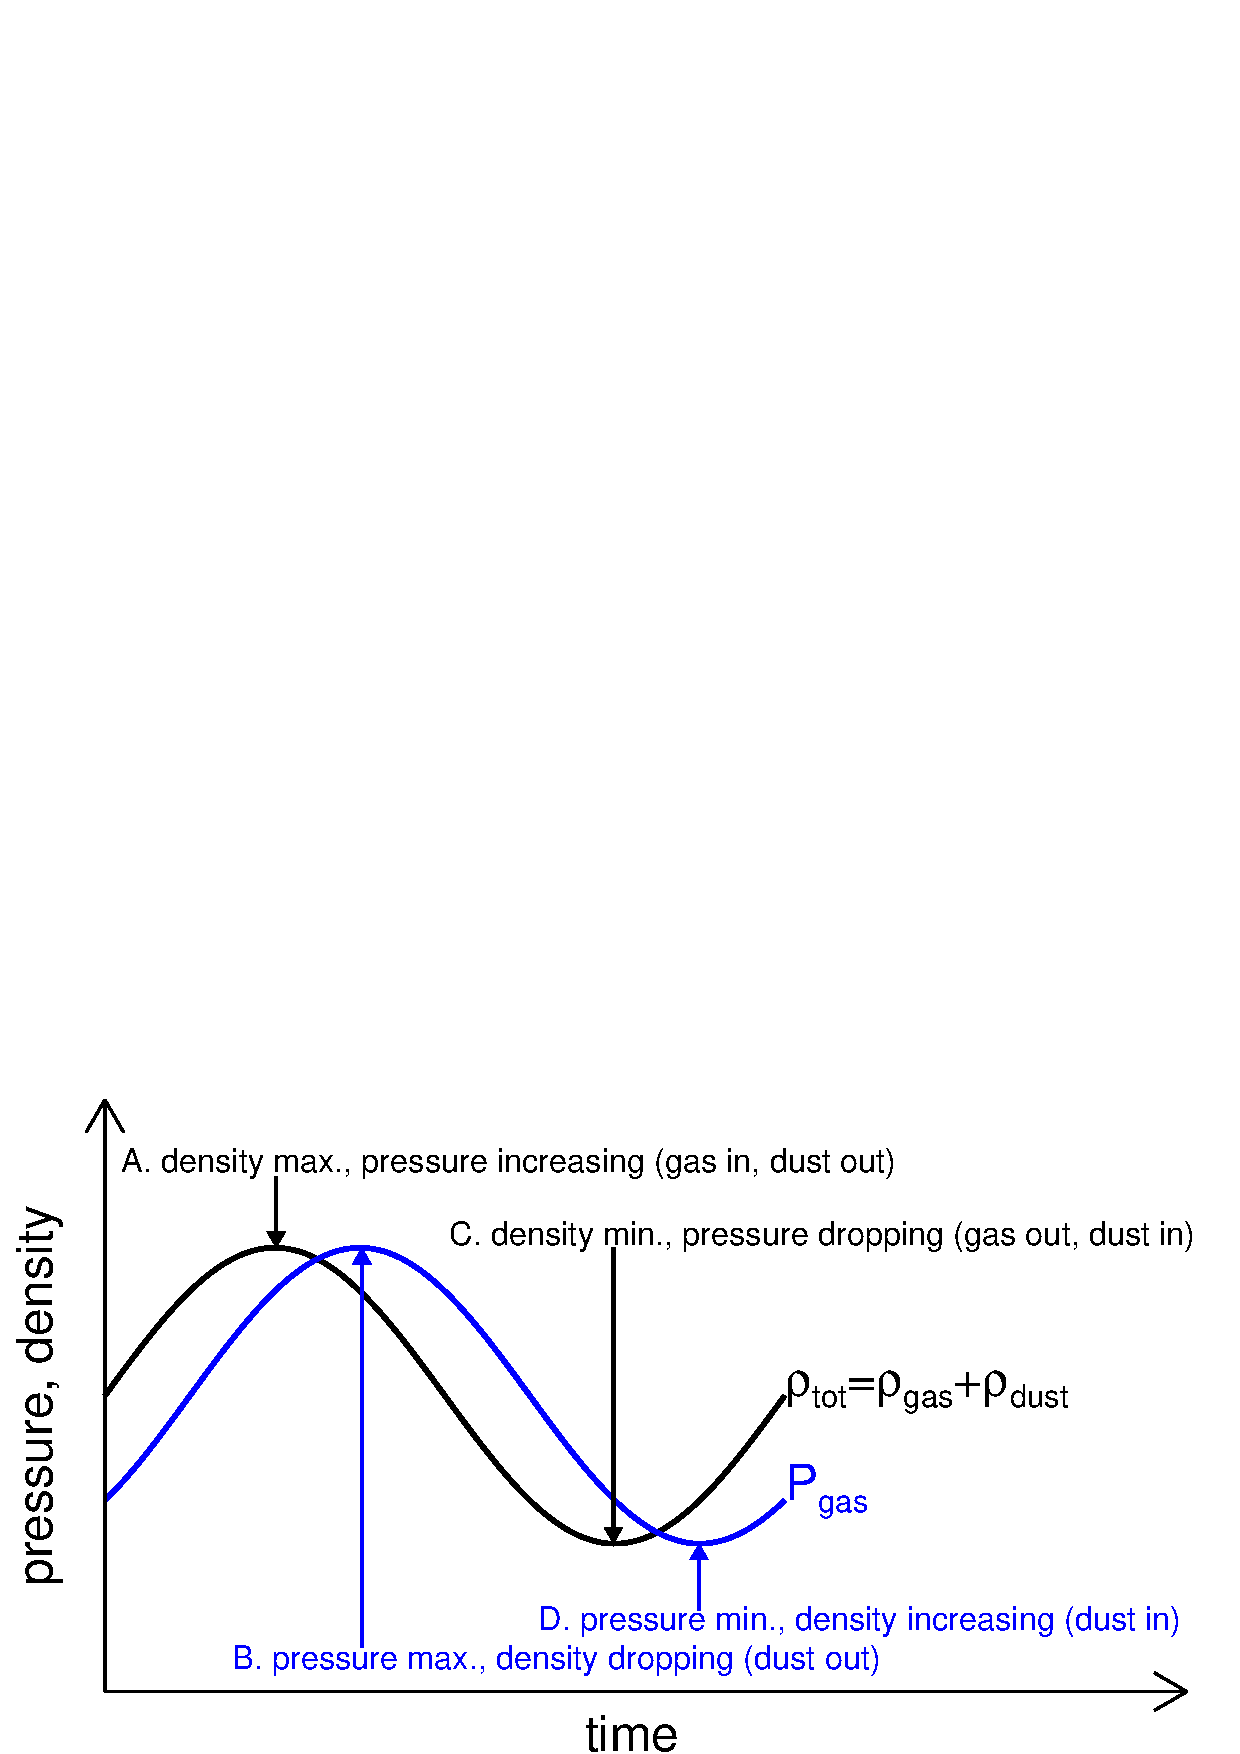
\includegraphics[width=\linewidth]{figures/drag}\\
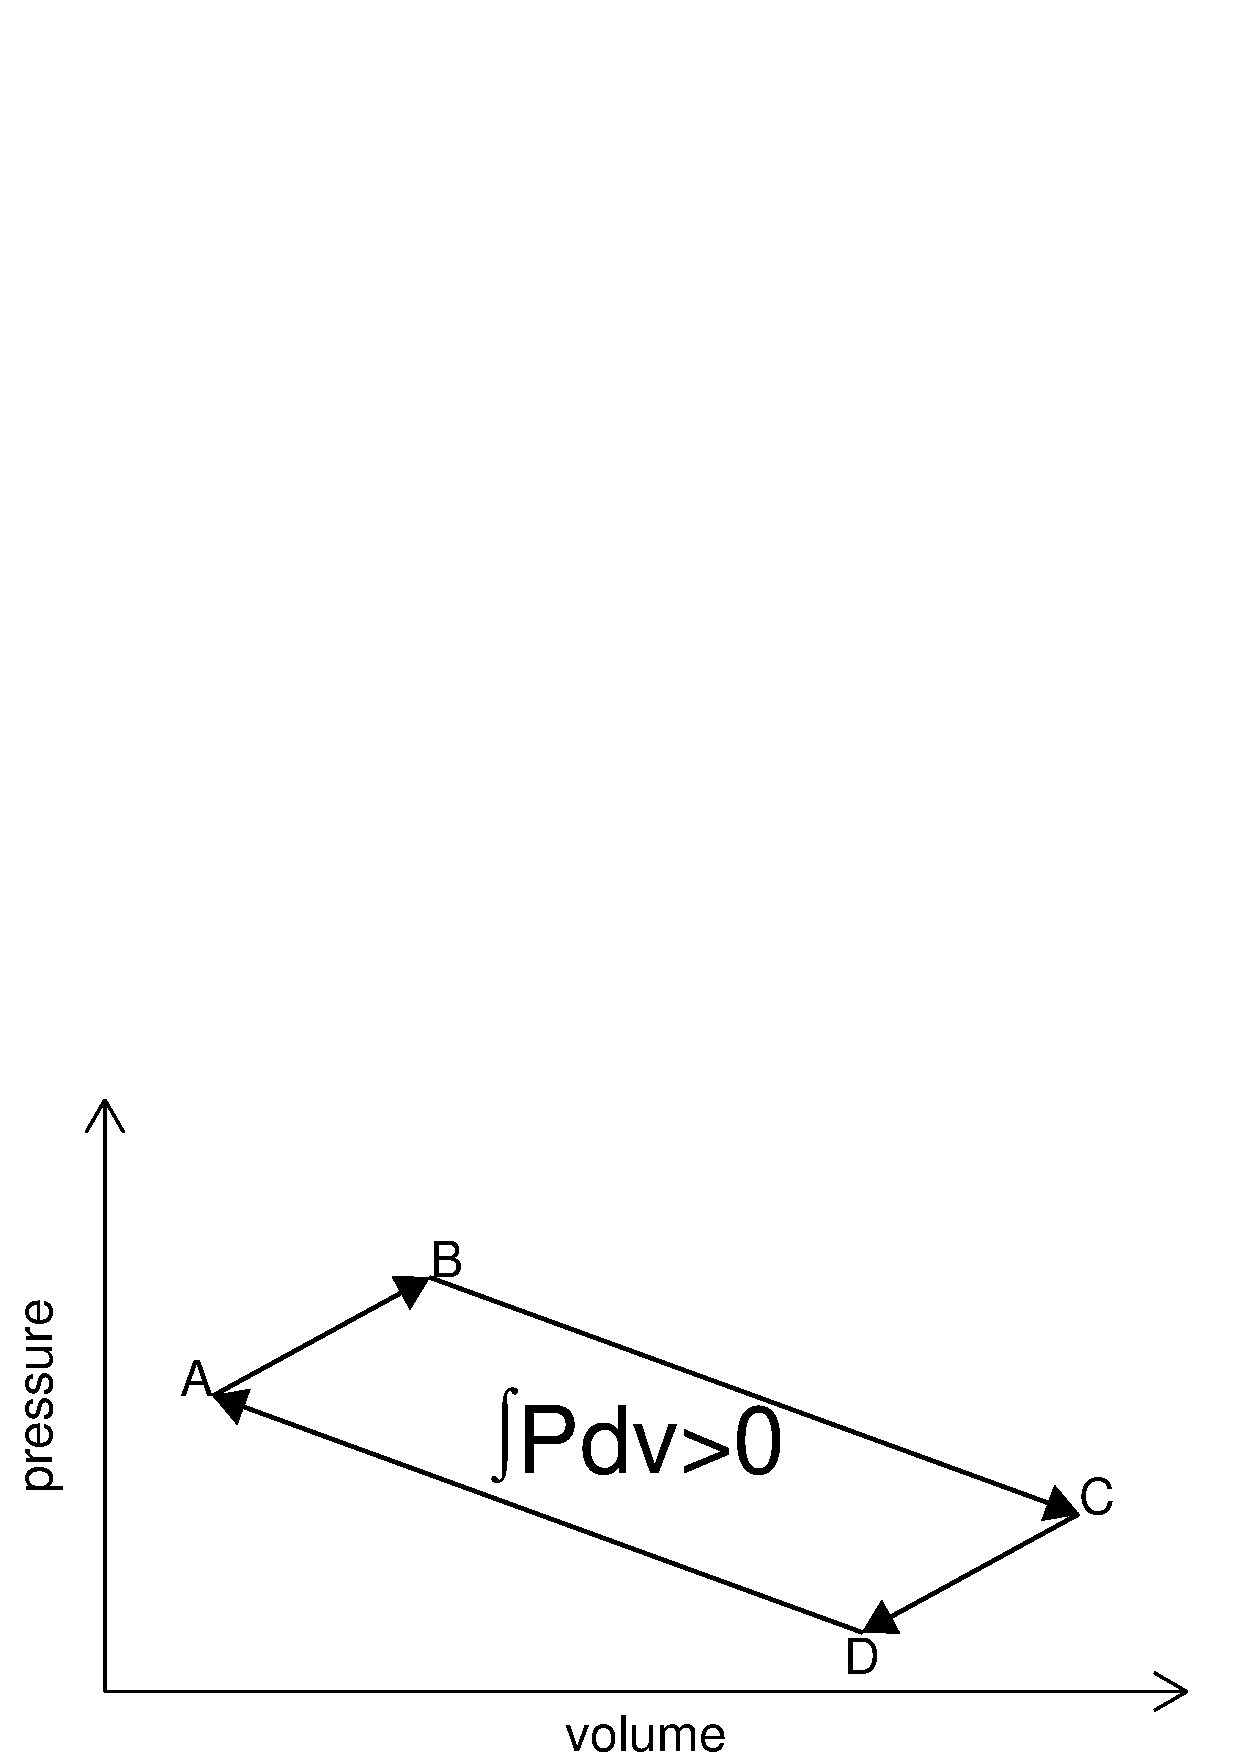
\includegraphics[width=\linewidth]{figures/pdv}
  \caption{Thermodynamic interpretation of overstable modes caused by
    dust-gas drag. Top: pressure and density evolution in time. 
    Bottom: oscillation cycle in the P-V plane. In the case shown,
    dust-drag causes 
    pressure to lag behind density, which results in a clockwise path in
    the P-V plane, implying positive work done by the fluid and
    hence would lead to growing oscillation amplitudes.  
    \label{pdv_cartoon}
  }
\end{figure}

This thermodynamic interpretation does not explain 
\emph{why} drag forces causes gas pressure to lag behind the dust
density, but merely shows 
that this \emph{must} be the case for any growing modes associated the
dust-gas drag. To rigorously understand how dust-drag causes this 
lag requires an explicit solution to the linearized equations with 
detailed treatment of the function $\mathcal{C}$. However, given the complexity of
$\mathcal{C}$ (see Appendix \ref{lin_dust}), we might generally expect
the dusty disks to  support a range of stable and unstable modes, with the
latter being associated with pressure-density lag. 

Indeed, \cite{jacquet11} explains the essence of the streaming 
instability in dusty protoplanetary disks as dust accumulation
(and hence compression) at a pressure bump, which then drags the 
gas towards it (and hence heating) to strengthen the pressure
bump. That is, heating occurs upon compression, as in stellar  
pulsational instabilities \citep{cox67}. In \S\ref{si} we check that the
streaming instability fits into this thermodynamic interpretation in
the strong drag limit.  

%A phase difference was also noted in the 
%numerical calculations of the streaming instability by 
%\citet{youdin07b}.    

%Whether the phase
%difference is positive or negative depends on the cooling function
%$\mathcal{C}$, but we may expect a system to generally have both
%modes, and that with a phase lag are unstable. 

\subsection{Locally isothermal gas perfectly coupled to dust}\label{dusty_vsi_int}
If $c_s(r,z)$ is non-uniform but $\tstop=0$, Eq. \ref{int_rel} 
gives  
\begin{align}
%  s = \frac{\imag\int P
%  \left(\nabla\cdot\dd\bm{v}^*\right)\left(\dd\bm{v}\cdot\nabla\ln{c_s^2}\right)dV}{2\omega\int\rho\left(|\dd 
%    v_r|^2 + |\dd v_z|^2\right)dV}. \label{vsi_check} 
  s = \frac{\imag\int P
    \left(\nabla\cdot\dd\bm{v}^*\right)\left(\dd\bm{v}\cdot\nabla\ln{c_s^2}\right)dV}{2\omega\mathcal{I}^2}. \label{vsi_check} 
\end{align} 
This is VSI caused by vertical shear arising from a radial
temperature gradient \citep{nelson13,barker15,lin15}. We present 
numerical solutions of the VSI with perfectly-coupled dust in \S\ref{results}. 
